\documentclass{beamer}
\mode<presentation>
\usepackage{amsmath}
\usepackage{amssymb}
%\usepackage{advdate}
\usepackage{adjustbox}
\usepackage{subcaption}
\usepackage{enumitem}
\usepackage{multicol}
\usepackage{mathtools}
\usepackage{listings}
\usepackage{xcolor}

\definecolor{mygray}{rgb}{0.5,0.5,0.5}
\definecolor{mymauve}{rgb}{0.58,0,0.82}
\definecolor{myblue}{rgb}{0.13,0.13,0.6}

\lstset{
	language=Python,
	backgroundcolor=\color{white},
	commentstyle=\color{mygray},
	keywordstyle=\color{myblue},
	numberstyle=\tiny\color{mygray},
	stringstyle=\color{mymauve},
	basicstyle=\ttfamily\small, % Change font size here
	breaklines=true,
	numbersep=8pt,
	showstringspaces=false,
	tabsize=4
}
\usepackage{url}
\def\UrlBreaks{\do\/\do-}
\usetheme{Boadilla}
\usecolortheme{lily}
\setbeamertemplate{footline}
{
  \leavevmode%
  \hbox{%
  \begin{beamercolorbox}[wd=\paperwidth,ht=2.25ex,dp=1ex,right]{author in head/foot}%
    \insertframenumber{} / \inserttotalframenumber\hspace*{2ex} 
  \end{beamercolorbox}}%
  \vskip0pt%
}
\setbeamertemplate{navigation symbols}{}

\providecommand{\nCr}[2]{\,^{#1}C_{#2}} % nCr
\providecommand{\nPr}[2]{\,^{#1}P_{#2}} % nPr
\providecommand{\mbf}{\mathbf}
\providecommand{\pr}[1]{\ensuremath{\Pr\left(#1\right)}}
\providecommand{\qfunc}[1]{\ensuremath{Q\left(#1\right)}}
\providecommand{\sbrak}[1]{\ensuremath{{}\left[#1\right]}}
\providecommand{\lsbrak}[1]{\ensuremath{{}\left[#1\right.}}
\providecommand{\rsbrak}[1]{\ensuremath{{}\left.#1\right]}}
\providecommand{\brak}[1]{\ensuremath{\left(#1\right)}}
\providecommand{\lbrak}[1]{\ensuremath{\left(#1\right.}}
\providecommand{\rbrak}[1]{\ensuremath{\left.#1\right)}}
\providecommand{\cbrak}[1]{\ensuremath{\left\{#1\right\}}}
\providecommand{\lcbrak}[1]{\ensuremath{\left\{#1\right.}}
\providecommand{\rcbrak}[1]{\ensuremath{\left.#1\right\}}}
\theoremstyle{remark}
\newtheorem{rem}{Remark}
\newcommand{\sgn}{\mathop{\mathrm{sgn}}}
\providecommand{\abs}[1]{\left\vert#1\right\vert}
\providecommand{\res}[1]{\Res\displaylimits_{#1}} 
\providecommand{\norm}[1]{\lVert#1\rVert}
\providecommand{\mtx}[1]{\mathbf{#1}}
\providecommand{\mean}[1]{E\left[ #1 \right]}
\providecommand{\fourier}{\overset{\mathcal{F}}{ \rightleftharpoons}}
%\providecommand{\hilbert}{\overset{\mathcal{H}}{ \rightleftharpoons}}
\providecommand{\system}{\overset{\mathcal{H}}{ \longleftrightarrow}}
	%\newcommand{\solution}[2]{\textbf{Solution:}{#1}}
%\newcommand{\solution}{\noindent \textbf{Solution: }}
\providecommand{\dec}[2]{\ensuremath{\overset{#1}{\underset{#2}{\gtrless}}}}
\newcommand{\myvec}[1]{\ensuremath{\begin{pmatrix}#1\end{pmatrix}}}
\newcommand{\mydec}[1]{\ensuremath{\begin{vmatrix}#1\end{vmatrix}}}
\let\vec\mathbf

\lstset{
%language=C,
frame=single, 
breaklines=true,
columns=fullflexible
}

\numberwithin{equation}{section}

\title{MATGEO: 1.1.6.19}
\author{Y Siddhanth \\ EE24BTECH11059\\ EE1030}

\date{\today} 
\begin{document}

\begin{frame}
\titlepage
\end{frame}

\section*{Outline}
\begin{frame}
\tableofcontents
\end{frame}
\section{Problem}
\begin{frame}
\frametitle{Problem Statement}
The vectors $\lambda\hat{i} + \hat{j} +2\hat{k}$, $\hat{i} + \lambda\hat{j} - \hat{k}$ and $2\hat{i} - \hat{j} +\lambda\hat{k}$  are coplanar if $\lambda = ?$
\end{frame}

\section{Solution}
\subsection{Information Table}
\begin{frame}
\frametitle{Information Table}
	\begin{table}[h!]    
		\centering
		

	\end{table}
\end{frame}
\subsection{Method of Solving}
\begin{frame}
	\frametitle{Method of Solving}
	The rank of a matrix $M$ is less than 3, then the matrix is coplanar. 
	\begin{align}
		Rank\brak{M} = 2\label{eq1.1.6.19.1}
	\end{align}
	Equivalently,
	\begin{align}
		\abs{M} = 0 \label{eq1.1.6.19.2}
	\end{align}
\end{frame}
\subsection{Finding $\lambda$ values}
\begin{frame}
\frametitle{Finding $\lambda$ values}
	\begin{align}
		\abs{M} = \myvec{\lambda & 1 & 2 \\ 1 & \lambda & -1 \\ 2 & -1 & \lambda} = 0 \label{eq1.1.6.19.3}
	\end{align}
	\begin{align}
		\lambda\brak{\lambda^2 - 1} - 1\brak{\lambda+2} + 2\brak{-1-2\lambda} = 0  \label{eq1.1.6.19.4}
	\end{align}
	\begin{align}
		\lambda^3 - 6\lambda - 4 = 0  \label{eq1.1.6.19.5}
	\end{align}
	\begin{align}
		\brak{\lambda + 2}\brak{\lambda^2 - 2\lambda - 2} = 0  \label{eq1.1.6.19.6}
	\end{align}
	\begin{align}
		\lambda = -2 \text{ or } \lambda = 1 \pm \sqrt{3}\label{eq1.1.6.19.6}
	\end{align}
\end{frame}
\subsection{Verifying Obtained Values}

\begin{frame}[fragile]
	\frametitle{Verifying Obtained Values}
	\begin{figure}[h]
		\centering
		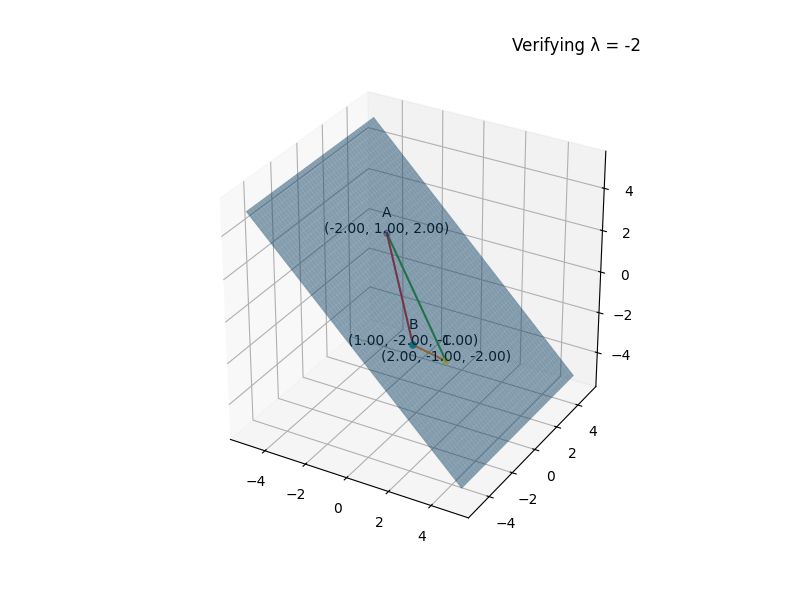
\includegraphics[width=0.7\linewidth]{figs/fig1.png}
		\caption{}
		\label{graph1}
	\end{figure}
\end{frame}

\begin{frame}[fragile]
	\frametitle{Verifying Obtained Values}
	\begin{figure}[h]
		\centering
		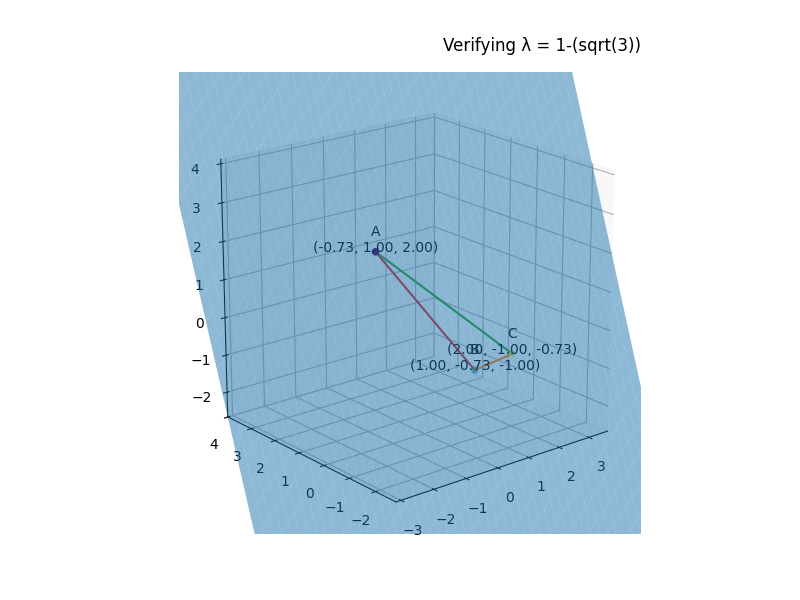
\includegraphics[width=0.7\linewidth]{figs/fig2.png}
		\caption{}
		\label{graph2}
	\end{figure}
\end{frame}

\begin{frame}[fragile]
	\frametitle{Verifying Obtained Values}
	\begin{figure}[h]
		\centering
		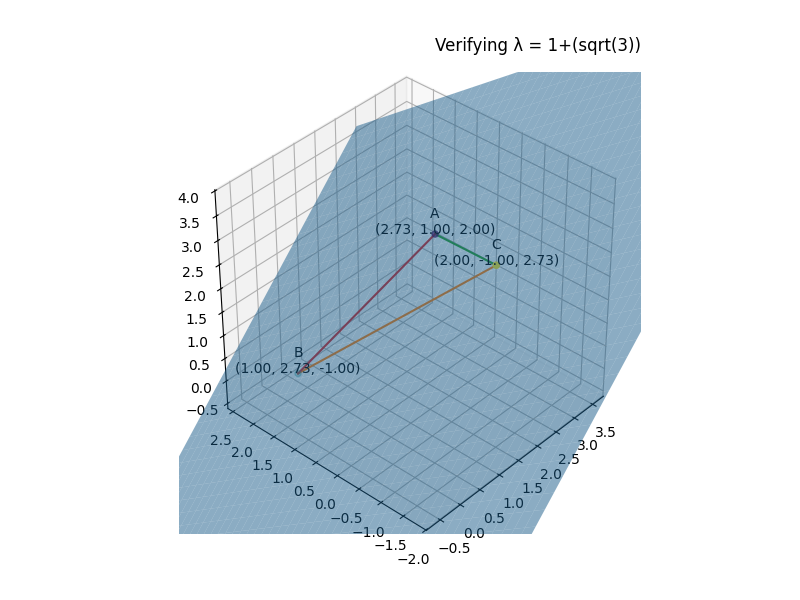
\includegraphics[width=0.7\linewidth]{figs/fig3.png}
		\caption{}
		\label{graph3}
	\end{figure}
\end{frame}
\subsection{$\lambda$ Verification Code}
\begin{frame}[fragile]
	\frametitle{$\lambda$ Verification Code}
	\begin{lstlisting}[mathescape=true]
		import sys                                          #for path to external scripts
		sys.path.insert(0, '/home/ysiddhanth/Documents/matgeo/codes/CoordGeo')        #path to my scripts
		import numpy as np
		import numpy.linalg as LA
		import matplotlib.pyplot as plt
		import matplotlib.image as mpimg
		from mpl_toolkits.mplot3d import Axes3D
		
		#local imports
		from line.funcs import *
		from triangle.funcs import *
		from conics.funcs import circ_gen
		roots = np.loadtxt("lambda.dat")
		#roots are roots[0] = -2; roots[1] and roots[2]
		k = roots[2]
		A = np.array(([k, 1,2])).reshape(-1,1) 
		B = np.array(([1,k, -1])).reshape(-1,1)  
		C = np.array(([2,-1, k])).reshape(-1,1)  
	\end{lstlisting}
\end{frame}
\begin{frame}[fragile]
	\frametitle{$\lambda$ Verification Code}
	\begin{lstlisting}[mathescape=true]
		P1 = np.array(([k, 1,2]))
		P2 = np.array(([1,k, -1]))
		P3 = np.array(([2,-1, k]))
		v1 = P2 - P1
		v2 = P3 - P1
		# Compute the normal vector (cross product of v1 and v2)
		normal = np.cross(v1, v2)
		# Plane equation: ax + by + cz = d
		# where [a, b, c] is the normal vector and d is calculated using one of the points
		a, b, c = normal
		d = np.dot(normal, P1)
		# Create a figure and a 3D Axes
		fig = plt.figure(figsize=(8, 6))
		ax = fig.add_subplot(111, projection='3d')
		# Generate grid points for x and y
		x = np.linspace(-5, 5, 50)
		y = np.linspace(-5, 5, 50)
		X, Y = np.meshgrid(x, y)
	\end{lstlisting}
\end{frame}
\begin{frame}[fragile]
	\frametitle{$\lambda$ Verification Code}
	\begin{lstlisting}[mathescape=true]
		# Calculate corresponding z values for each (x, y) pair to satisfy the plane equation
		Z = (-a*X - b*Y - d) / c
		# Plot the plane
		ax.plot_surface(X, Y, Z, alpha=0.5)
		#Generating all lines
		x_BC = line_gen(B,C)
		x_AB = line_gen(A,B)
		x_AC = line_gen(A,C)
		#Plotting all lines
		ax.plot(x_BC[0,:],x_BC[1,:], x_BC[2,:],label='$BC$')
		ax.plot(x_AC[0,:],x_AC[1,:], x_AC[2,:],label='$AC$')
		ax.plot(x_AB[0,:],x_AB[1,:], x_AB[2,:],label='$AB$')
		# Scatter plot
		colors = np.arange(2, 5)  # Example colors
		tri_coords = np.block([A, B, C])  # VStack A, B, C
		ax.scatter(tri_coords[0, :], tri_coords[1, :], tri_coords[2, :], c=colors)
		vert_labels = ['A', 'B', 'C']
	\end{lstlisting}
\end{frame}
\begin{frame}[fragile]
	\frametitle{$\lambda$ Verification Code}
	\begin{lstlisting}[mathescape=true]
		for i, txt in enumerate(vert_labels):
		# Annotate each point with its label and coordinates
		ax.text(tri_coords[0, i], tri_coords[1, i], tri_coords[2, i], f'{txt}\n({tri_coords[0, i]:.02f}, {tri_coords[1, i]:.02f}, {tri_coords[2, i]:.02f})',
		fontsize=10, ha='center', va='baseline')
		ax.spines['top'].set_color('none')
		ax.spines['left'].set_position('zero')
		ax.spines['right'].set_color('none')
		ax.spines['bottom'].set_position('zero')
		# Set limits and aspect ratio to magnify the plane
		ax.set_xlim(-4, 4)  # Adjust limits based on your data
		ax.set_ylim(-4, 4)  # Adjust limits based on your data
		ax.set_zlim(-4, 4)  # Adjust limits based on your data
		ax.set_box_aspect([1,1,1])  # Equal aspect ratio for x, y, and z axes
		plt.grid() # minor
		plt.axis('equal')
		plt.show()
	\end{lstlisting}
\end{frame}

\subsection{Methods of Finding $\lambda$}
\begin{frame}[fragile]
	\frametitle{Methods of Finding $\lambda$}
	\textbf{Method 1(using sympy) : } Use sympy to find the det and solve for lambda.
	\begin{lstlisting}[mathescape=true]
		import sympy as sp
		$\lambda$ = sp.symbols('$\lambda$')
		A = sp.Matrix([[$\lambda$, 1, 2], [1, $\lambda$, -1], [2, -1, $\lambda$]])
		det_A = A.det()
		lambda_solutions = sp.solve(det_A, $\lambda$)
		numeric_solutions = [sp.N(sol) for sol in lambda_solutions]
	\end{lstlisting}
		
\end{frame}
\begin{frame}[fragile]
	\frametitle{Methods of Finding $\lambda$}
	\textbf{Method 2(using numpy) : } 
	\begin{align}
		\abs{M} = \myvec{\lambda & 1 & 2 \\ 1 & \lambda & -1 \\ 2 & -1 & \lambda} = \myvec{0 & 1 & 2 \\ 1 & 0 & -1 \\ 2 & -1 & 0} + \lambda I = \abs{A + \lambda I}
	\end{align}
	Thus, the values of $\lambda$ are the negative of the eigen values of the matrix $A$.\\
	\begin{lstlisting}[mathescape=true]
		import numpy as np
		A = np.array([[0, 1, 2], [1, 0. -1], [2, -1, 0]])
		eigenvalues = np.linalg.eigvals(A)
		$\lambda$-vals = -eigenvals
	\end{lstlisting}
\end{frame}

\end{document}
